% Midterm report draft. Paste into the course Overleaf template (NeurIPS style)
% and upload figures/dp_by_type.pdf. Items marked \todo{} are open.
\documentclass{article}
\usepackage[final]{neurips_2019}
\usepackage[utf8]{inputenc}
\usepackage[T1]{fontenc}
\usepackage{hyperref}
\usepackage{url}
\usepackage{booktabs}
\usepackage{amsmath}
\usepackage{amsfonts}
\usepackage{graphicx}
\usepackage{xcolor}
\newcommand{\todo}[1]{\textcolor{red}{[TODO: #1]}}

\title{Learning to Pick the Plan: A Learned Trajectory Scorer\\for Diffusion-Based Driving Planners\\(Midterm Report)}

\author{Risha Ranjan \And Shubham Saboo \And Neha Kayiti \And Kaushal Jadhav \\
Carnegie Mellon University \\
\texttt{\{rishar, spsaboo, nkayiti, ksjadhav\}@andrew.cmu.edu}}

\begin{document}
\maketitle

\begin{abstract}
Many learning-based planners for self-driving cars generate several candidate trajectories and then choose one, and the strongest systems still make that final choice with hand-written rules. We are building a learned scorer for Diffusion Planner~\cite{zheng2025diffusion} that predicts how safe and useful each candidate trajectory is and selects the best one. Labels come from a rule-based evaluator run on real driving logs. As a first step, we reproduced the released Diffusion Planner in nuPlan's closed-loop simulator on the Test14-hard benchmark. It scores 74.63 with non-reactive traffic and 68.63 with reactive traffic, within 1.4 points of the published results (75.99 and 69.22). This report describes the reproduction, the scorer design, and the remaining work.
\end{abstract}

%-------------------------------------------------------------------------
\section{Overview and context}

\paragraph{Motivation.}
Learning-based planners can produce flexible, human-like driving, but on standard benchmarks the top results still come from hybrid systems in which a rule-based module checks or selects the final trajectory~\cite{zheng2025diffusion,cheng2024pluto}. These rules can miss situations their designers did not anticipate, and they are slow because they simulate every candidate. Replacing this step with a learned model could make the planner more data-driven and better in rare or difficult scenarios. That would matter to anyone deploying learned planners.

\paragraph{Objectives.}
Our question is whether a learned scorer can choose trajectories as well as, or better than, hand-written rules, and when each one fails. Our quantitative objectives are:
(i) match or exceed the closed-loop score (CLS) of a rule-based selector on Test14-hard, in both non-reactive (NR) and reactive (R) traffic;
(ii) select trajectories faster than the rule-based selector; and
(iii) test whether a hybrid of learned and rule-based scores beats both.

%-------------------------------------------------------------------------
\section{Related work and background}

\paragraph{Literature review.}
\emph{Generative planners.} Diffusion Planner~\cite{zheng2025diffusion} and Flow Planner~\cite{tan2025flow} produce diverse trajectories with diffusion or flow matching, but reach their best scores only with rule-based refinement.
\emph{Candidate selection.} PLUTO~\cite{cheng2024pluto} generates many candidates and selects among them with a mix of learned confidence and a rule-based check. Hydra-MDP~\cite{li2024hydra} and GTRS~\cite{li2025gtrs} train neural scorers that predict rule-based driving metrics for a set of trajectories. GTRS shows that such a scorer can rank trajectories it never saw during training. Our project applies this learned-scoring idea to the candidates of a diffusion planner.

\paragraph{Background.}
Our rule-based reference is PDM-Closed~\cite{dauner2023parting}, which won the 2023 nuPlan challenge. It simulates each candidate and scores it on collisions, drivable-area compliance, progress, and comfort. Its scoring function is also our source of training labels. We evaluate on Test14-hard, introduced by PlanTF~\cite{cheng2024plantf}: 272 scenarios across 14 scenario types, chosen as the cases where PDM-Closed performs worst.

%-------------------------------------------------------------------------
\section{Methodology}

\paragraph{Base planner.}
Diffusion Planner~\cite{zheng2025diffusion} is a diffusion-transformer planner that jointly denoises the future trajectories of the ego vehicle and nearby agents. Its inputs, in the ego frame, are: the past 2\,s (21 frames at 10\,Hz) of up to 32 neighboring agents ($32\times21\times11$); 5 static objects ($5\times10$); 70 lane segments ($70\times20\times12$, i.e., 20 points per lane with 12 features per point); and 25 route lanes ($25\times20\times12$). It outputs 8\,s (80 steps) of future trajectory for the ego vehicle and the 10 nearest agents. The encoder and decoder each have 3 transformer layers, with hidden size 192 and 6 attention heads. Because sampling is stochastic, repeated sampling (or guidance) yields a set of $K$ candidate trajectories for the same scene.

\paragraph{Proposed scorer.}
The scorer reuses Diffusion Planner's scene encoder. Each of the $K$ candidate ego trajectories ($K\times80\times4$: $x$, $y$, $\cos\theta$, $\sin\theta$) is embedded with a small MLP into one token. A lightweight transformer then lets each candidate token attend to the scene tokens and to the other candidates. Per-metric heads output, for each candidate, the predicted probability of each PDM sub-metric: no at-fault collision, drivable-area compliance, driving-direction compliance, and making progress, plus the weighted time-to-collision, progress, and comfort terms. The predicted metrics are combined with the same formula as the CLS (Eq.~\ref{eq:cls}), and the highest-scoring candidate is executed. The hybrid variant uses $s = \lambda\,s_{\text{learned}} + (1-\lambda)\,s_{\text{PDM}}$. \todo{Insert architecture diagram (scene encoder $\rightarrow$ candidate tokens $\rightarrow$ transformer $\rightarrow$ metric heads), with tensor shapes.}

\paragraph{Dataset.}
We use nuPlan~\cite{caesar2021nuplan}, a large real-world driving dataset with a closed-loop simulator. Evaluation uses the nuPlan v1.1 test split, filtered to the Test14-hard scenarios. Because nuPlan provides no scores for alternative trajectories, we generate our own labels. The steps are:
(1) sample a subset of \todo{N} scenarios from the training split;
(2) run the frozen Diffusion Planner to produce $K=$\todo{K} candidates per scene;
(3) score each candidate with the PDM-Closed scorer, using the logged future motion of other agents; and
(4) store (scene features, candidates, per-metric labels) for training.
\todo{Fill in subset size, $K$, sampling scheme, train/val split, storage format, and the batch construction (one scene with its $K$ candidates per sample).}

\paragraph{Evaluation metric.}
Our main metric is nuPlan's closed-loop score. For each scenario,
\begin{equation}
\text{CLS} = \underbrace{\prod_{m\in\mathcal{M}} m}_{\text{multipliers}} \cdot \frac{5\,\text{TTC} + 5\,\text{EP} + 4\,\text{SL} + 2\,\text{C}}{16},
\label{eq:cls}
\end{equation}
where $\mathcal{M}$ contains no at-fault collision, drivable-area compliance, driving-direction compliance, and making progress. TTC is time-to-collision within bound, EP is ego progress along the expert route, SL is speed-limit compliance, and C is comfort. The benchmark score is the mean CLS over scenarios, scaled to 0--100. We report it with non-reactive (log-replay) and reactive (IDM) agents. As offline diagnostics, we will also report top-1 accuracy and regret against the best candidate under the PDM labels, along with selection latency.

\paragraph{Loss function.}
Each binary metric head is trained with binary cross-entropy, and each continuous head with binary cross-entropy against its soft label in $[0,1]$. The total loss is a weighted sum over metric heads. \todo{Confirm the loss weights and optimizer once training starts.}

\paragraph{Experimental iterations so far.}
We completed two full closed-loop runs of the baseline (NR and R, 272 scenarios each), preceded by 5-scenario smoke tests to validate the pipeline. \todo{Add the PDM-Closed reference run and/or the candidate-headroom experiment (Section~\ref{sec:next}) as further iterations.}

%-------------------------------------------------------------------------
\section{Baseline and extensions}

\paragraph{Baseline selection.}
Baseline (1) is Diffusion Planner without any selection step: the released checkpoint, run as published. It is the model our scorer builds on, so any gain from the scorer is measured against it. The paper's second variant, with rule-based refinement, is not in the public release; the authors used the refinement module of State Transformer~2~\cite{dp_issue14}. \todo{State the decision for baseline (2): we propose to select among $K$ sampled Diffusion Planner candidates with the PDM-Closed scorer. This is the rule-based selector that our learned scorer is meant to replace, and it scores the same candidate set.} PDM-Closed alone is reported as a rule-based reference.

\paragraph{Implementation.}
We pinned nuplan-devkit, Diffusion Planner, and tuplan\_garage to fixed commits and wrote scripts for environment setup, data download, simulation, and result aggregation. Simulations ran on AWS (\todo{instance type, GPU, vCPUs, RAM, parallel workers}). Each 272-scenario run took \todo{wall-clock time}.

\begin{table}[t]
\centering
\caption{Diffusion Planner (no refinement) on Test14-hard, 272 scenarios per run. CLS on a 0--100 scale; sub-metrics are averages in \%.}
\label{tab:baseline}
\small
\begin{tabular}{lcc}
\toprule
 & NR & R \\
\midrule
CLS (ours)                     & \textbf{74.63} & \textbf{68.63} \\
CLS (published~\cite{zheng2025diffusion}) & 75.99 & 69.22 \\
$\Delta$                       & $-1.36$ & $-0.59$ \\
\midrule
No at-fault collision          & 86.8 & 86.6 \\
Drivable-area compliance       & 95.2 & 95.2 \\
Driving-direction compliance   & 98.9 & 98.9 \\
Making progress                & 98.5 & 92.3 \\
Time-to-collision within bound & 76.8 & 80.5 \\
Speed-limit compliance         & 96.5 & 97.4 \\
Progress along expert route    & 89.7 & 76.7 \\
Comfort                        & 91.9 & 86.0 \\
\bottomrule
\end{tabular}
\end{table}

\begin{figure}[t]
\centering
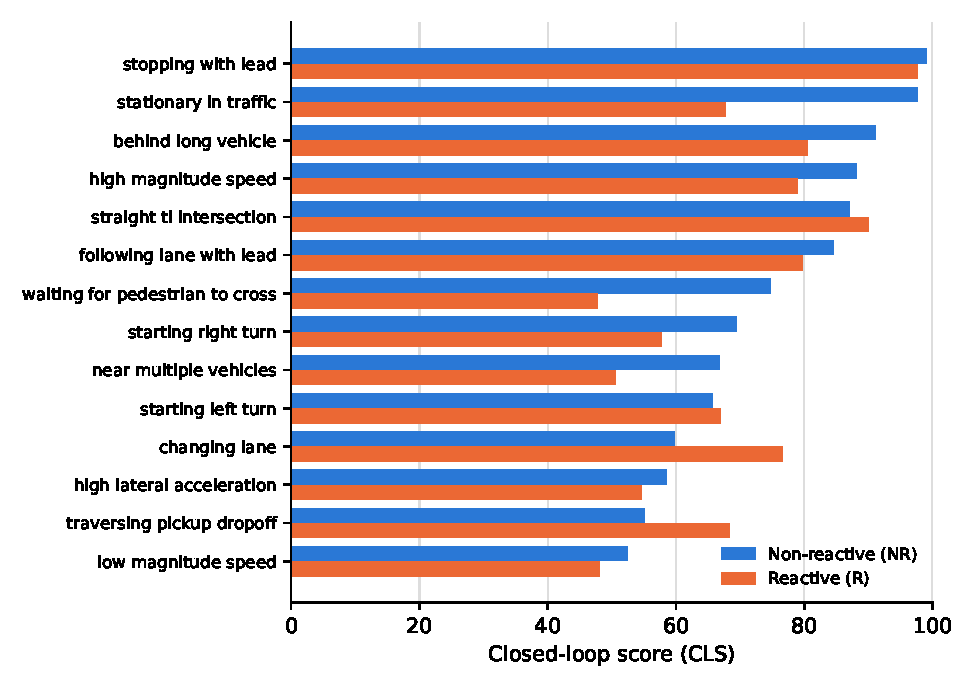
\includegraphics[width=0.85\linewidth]{figures/dp_by_type.pdf}
\caption{Diffusion Planner CLS by scenario type on Test14-hard, with non-reactive and reactive agents.}
\label{fig:bytype}
\end{figure}

\paragraph{Baseline reproduction evidence.}
Table~\ref{tab:baseline} shows that our CLS is within 1.4 (NR) and 0.6 (R) points of the published numbers. Possible sources of the gap are stochastic diffusion sampling (we ran one seed per setting), upstream code changes since publication, and differences in library versions and hardware. \todo{Add a second seed if budget allows, to estimate run-to-run variance.}

\paragraph{Planned extensions.}
(1) A learned scorer that replaces the rule-based selector.
(2) A hybrid scorer that combines learned and rule-based scores, with $\lambda$ swept.
We will also vary the training candidates (a fixed trajectory vocabulary vs.\ planner samples) and whether the scene encoder is frozen or fine-tuned.

%-------------------------------------------------------------------------
\section{Preliminary results}

Figure~\ref{fig:bytype} breaks the baseline down by scenario type. The weakest types in both settings are \emph{low magnitude speed} (52.4 NR / 48.1 R), \emph{high lateral acceleration} (58.5 / 54.6), and \emph{traversing pickup/dropoff} (55.1 NR). With reactive agents, the largest drops are in \emph{waiting for pedestrian to cross} ($74.8\rightarrow47.8$), \emph{stationary in traffic} ($97.7\rightarrow67.7$), and \emph{near multiple vehicles} ($66.8\rightarrow50.6$). Table~\ref{tab:baseline} shows that these drops come mostly from lower progress along the expert route ($89.7\rightarrow76.7$) and more frequent failures to make progress, not from more collisions (86.8 vs.\ 86.6). This suggests the planner becomes overly hesitant when other agents respond to it. A selector that can trade a small amount of safety margin for progress, chosen per scene, is the kind of decision a learned scorer could make better than a fixed output. These scenario types are where we expect the largest gains, and we will report results broken down by them.
\todo{If the headroom experiment is done: report how often the best of $K$ candidates (under PDM labels) beats the default output, as an upper bound on what selection can gain.}

%-------------------------------------------------------------------------
\section{Discussion: challenges and risks}

\paragraph{Challenges so far.}
(1) The rule-based refinement variant of Diffusion Planner is not public, so the second baseline has to be redefined (Section~4).
(2) Compute moved from the Pittsburgh Supercomputing Center, planned in the proposal, to AWS course credits (about \$150 per member). We therefore evaluate on subsets during development and run full benchmarks only for final comparisons.
(3) Setting up nuPlan (dataset licensing, large downloads, simulator dependencies) took a large share of the time before the midterm.

\paragraph{Risks.}
(1) Label generation runs the PDM scorer on $K$ candidates for every training scene and may be expensive; we will start from a small subset and scale up.
(2) Training on a subset may yield lower absolute scores than the original papers. We mitigate this by comparing every method under the same setup.
(3) Val14 requires the validation split, which we have not downloaded yet. \todo{Decide whether Val14 is in scope for the final report.}

%-------------------------------------------------------------------------
\section{Next steps}
\label{sec:next}
\begin{enumerate}
\item Implement baseline (2): PDM-scorer selection over $K$ Diffusion Planner samples; run Test14-hard NR/R. Also run PDM-Closed as a reference.
\item Candidate-headroom study on a subset: the gap between the default output and the best of $K$ candidates.
\item Label-generation pipeline on a training subset (\todo{owner}).
\item Train a first scorer with offline top-1/regret evaluation, then closed-loop evaluation.
\item Hybrid scorer and ablations (candidate source, frozen vs.\ fine-tuned encoder, $\lambda$).
\end{enumerate}
\todo{Add dates/owners per item.}

\paragraph{Team contributions.}
\todo{Update: e.g., Shubham: setup scripts / dataset; Risha: baseline simulation runs; Neha: label generation; Kaushal: evaluation scripts, analysis, report.}

\begin{thebibliography}{99}\small
\bibitem{caesar2021nuplan} H.~Caesar et al. nuPlan: A closed-loop ML-based planning benchmark for autonomous vehicles. In \emph{CVPR Workshops}, 2021.
\bibitem{cheng2024plantf} J.~Cheng, Y.~Chen, X.~Mei, B.~Yang, B.~Li, and M.~Liu. Rethinking imitation-based planners for autonomous driving. In \emph{ICRA}, 2024.
\bibitem{cheng2024pluto} J.~Cheng, Y.~Chen, and Q.~Chen. PLUTO: Pushing the limit of imitation learning-based planning for autonomous driving. arXiv:2404.14327, 2024.
\bibitem{dauner2023parting} D.~Dauner, M.~Hallgarten, A.~Geiger, and K.~Chitta. Parting with misconceptions about learning-based vehicle motion planning. In \emph{CoRL}, 2023.
\bibitem{li2024hydra} Z.~Li et al. Hydra-MDP: End-to-end multimodal planning with multi-target hydra-distillation. arXiv:2406.06978, 2024.
\bibitem{li2025gtrs} Z.~Li et al. Generalized trajectory scoring for end-to-end multimodal planning. arXiv:2506.06664, 2025.
\bibitem{tan2025flow} T.~Tan, Y.~Zheng, et al. Flow matching-based autonomous driving planning with advanced interactive behavior modeling. In \emph{NeurIPS}, 2025.
\bibitem{zheng2025diffusion} Y.~Zheng, R.~Liang, K.~Zheng, et al. Diffusion-based planning for autonomous driving with flexible guidance. In \emph{ICLR}, 2025.
\bibitem{dp_issue14} Diffusion-Planner GitHub issue \#14: refinement module. \url{https://github.com/ZhengYinan-AIR/Diffusion-Planner/issues/14}.
\end{thebibliography}

\end{document}
